\documentclass[paper=a4, fontsize=11pt]{jhwhw} % A4 paper and 11pt font size
\usepackage{amsmath,amsfonts,amsthm, amssymb} % Math packages
\setlength\parindent{0pt} % Removes all indentation from paragraphs - comment this line for an assignment with lots of text
\usepackage{graphicx}
\usepackage{verbatim}
\usepackage{enumerate}
\usepackage{mathtools}
\usepackage{color}
\newcommand\SetSymbol[1][]{\:#1\vert\:}
\providecommand\given{} % to make it exist
\DeclarePairedDelimiterX\Set[1]\{\}{\renewcommand\given{\SetSymbol[\delimsize]}#1}
\usepackage{listings}

\definecolor{dkgreen}{rgb}{0,0.6,0}
\definecolor{gray}{rgb}{0.5,0.5,0.5}
\definecolor{mauve}{rgb}{0.58,0,0.82}

\lstset{frame=tb,
    language=Java,
    aboveskip=3mm,
    belowskip=3mm,
    showstringspaces=false,
    columns=flexible,
    basicstyle={\small\ttfamily},
    numbers=none,
    numberstyle=\tiny\color{gray},
    keywordstyle=\color{blue},
    commentstyle=\color{dkgreen},
    stringstyle=\color{mauve},
    breaklines=true,
    breakatwhitespace=true,
    tabsize=3
}



\begin{document}
\title{MP1}
\author{Ben Haines}

\section{Part 1}
\subsection{Normalization Implementation}
\begin{lstlisting}
public String Normalization(String token) {
    // remove all English punctuation
    token = token.replaceAll("\\p{Punct}+", "");
    // convert to lower case
    token = token.toLowerCase();

    //Note that this doesn't attempt to recognize doubles
    //This is because all periods were removed in the previous step.
    //At this point in the processing a double looks the same as an int.
    token = token.replaceAll("\\d+", "NUM");

    return token;
}
\end{lstlisting}

\subsection{Graphs}
\begin{figure}[ht]
    \center
    \caption{Total Term Frequency}
    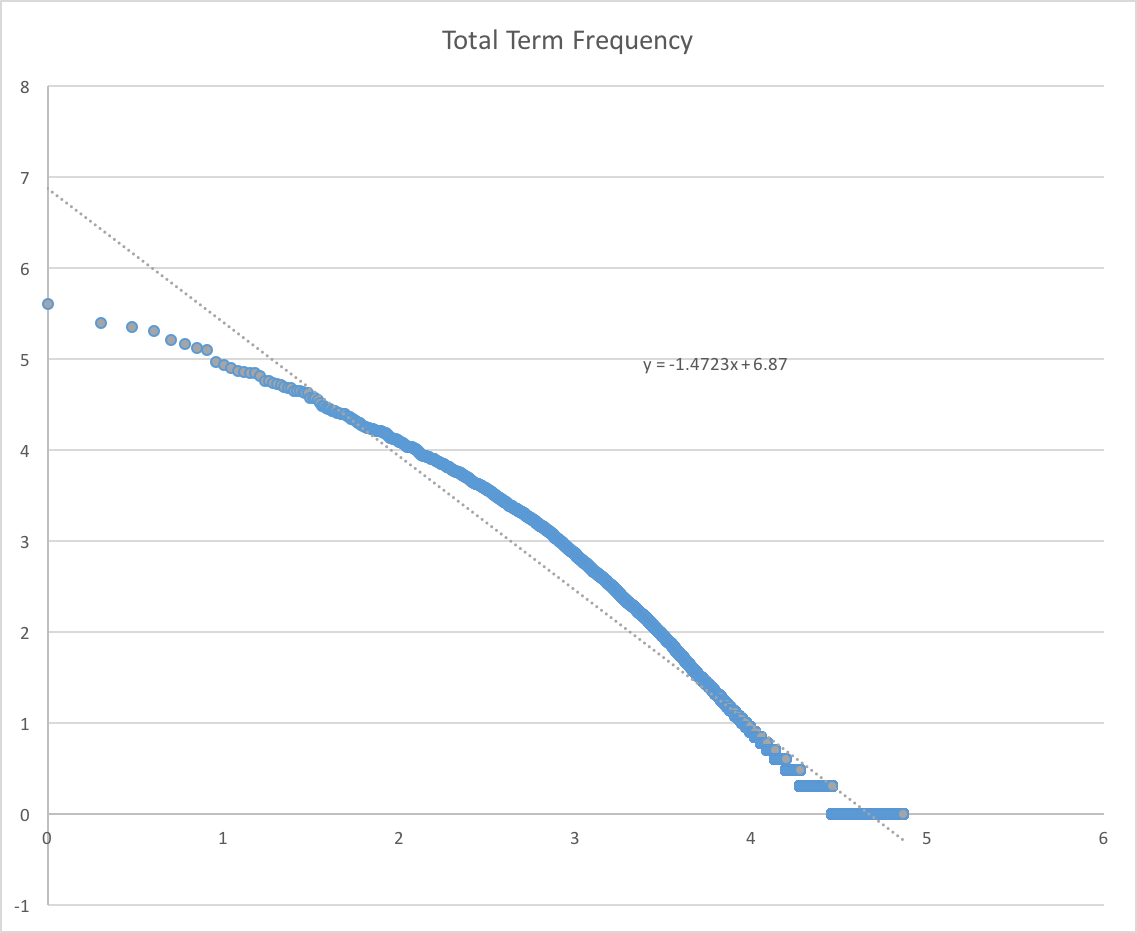
\includegraphics[scale=.71]{Picture1}
\end{figure}
The y-axis on the above graph is total term frequency. The x-axis is rank of the word by total term frequency. Both axes are log scaled.

\section{Part 2}
\subsection{Restaurant Specific Stopwords}
It was unclear to me at what point in the process we were intended to remove stopwords. My interpretation of the instructions was that we should find the top hundred N-grams in the Yelp data set and from these remove the stopwords that already appeared in the generic stopwords list. This left me with the following 33 N-grams with the highest document frequency that were not located in the generic stopwords list. For each N-gram their document frequency in the Yelp corpus is listed to the right. 
\begin{verbatim}
nt,17832.0
good,17592.0
food,16661.0
NUM,15831.0
great,13524.0
and the,12279.0
order,11857.0
of the,11752.0
it was,11618.0
time,11260.0
this place,9925.0
wait,9787.0
servic,9360.0
back,9347.0
it s,9247.0
in the,9105.0
friend,9070.0
love,9014.0
fri,8637.0
and i,8291.0
on the,8291.0
the food,8180.0
delici,7802.0
ve,7619.0
sauc,7503.0
restaur,7442.0
i was,7277.0
do nt,7192.0
dish,6936.0
eat,6929.0
for a,6862.0
\end{verbatim}

It's interesting to see what things are specific to the Yelp review corpus. Some of the words are predictable results of properties of the dataset. Things like "good", "food", "eat", "delici", and "restaur" make sense in the context of restaurant reviews. Other terms seem to be a result of the particular way the data was processed rather than any characteristic of the data itself. The 2-grams "of the", "it was", and "and the" are simply combinations of two stopwords. Later when I filter stopwords out of the vocabulary I check if either token in a given 2-gram is a stopword and remove it if it is. This means that the addition of things like "it was" and "of the" to the stopword list is redundant and doesn't provide any extra filtering. Other terms like "nt" and "ve" seem to tell us something about the tokenizing process. The only reasonable source of these tokens that I can determine is from contractions like "they've", "didn't", and so on. It's interesting that these are separated into separate tokens, 

"NUM" is another interesting case that results from the method of processing. It makes sense that numbers should be common in the context of restaurant reviews. They could come up in things like price, the amount of time spent waiting for service, or the number of options on the menu. Obviously "NUM" as a string is not very common in english text so this is a good example of how merging the retaurant stopwords and the generic stopwords provides extra utility. 

\subsection{Size of Vocabulary}
The final size of my controlled vocabulary was 3538 uniqe N-grams. 

I thought that this number was surprisingly low. Considering that there were over thirty thousand reviews, each presumably a few sentences long, I was expecting there to be a similarly large resulting vocabulary. Part of the reason the vocabulary is so small is a result of my aggressive stopword filtering method mentioned above. A less aggressive approach would be to only filter out 2-grams for which each individual token is a stopword rather than filtering all 2-grams where either token is a stopword. It would be interesting to compare the results of the two approaches. Filtering fewer N-grams from the vocabulary would on the one hand decrease the specificity of the information known about each document but on the other hand might include useful information to assist in making similarity measures. 

\subsection{Top \& Bottom Fifty}
The top fifty N-grams from the controlled vocabulary and their corresponding inverse document frequency scores were:
\begin{verbatim}
tabl,2.744802486140284
make,2.779275682227886
menu,2.847732627506703
chees,2.8528300651659926
tast,2.856794391467902
chicago,2.893198815895139
amaz,2.894916734201164
thing,2.9030307191576297
nice,2.9249364404418143
peopl,2.9591801900089854
pretti,2.960464476030845
seat,2.969871536086873
night,2.9882000835825044
perfect,3.052310861812199
recommend,3.0628308860025797
drink,3.081718739641433
flavor,3.0846245117150657
price,3.1165140262948277
bar,3.116943302970233
meal,3.117802409552282
small,3.147681417759915
dinner,3.151452077656108
favorit,3.1601565182862545
bit,3.162625378254233
worth,3.1684852102123484
made,3.218066826738092
enjoy,3.2413767851840953
side,3.24429862802246
experi,3.2464956263430023
chicken,3.2513951951841604
long,3.2659903831476025
pizza,3.2742476551360356
top,3.2838412657018536
fresh,3.2838412657018536
star,3.3071966195996105
line,3.3110993174111902
serv,3.3252765041961165
review,3.3271290917313943
lot,3.3480077944778874
day,3.352073391621496
plate,3.354248487639448
atmospher,3.3649203634468994
sweet,3.392250564209039
ll,3.3936651916906686
minut,3.409359621406658
tasti,3.4148390871712833
ca,3.4394304903086055
staff,3.4698224789133385
expect,3.4701280556918817
visit,3.4787223381792156
\end{verbatim}

The bottom fifty N-grams from the controlled vocabulary and their corresponding inverse document frequency scores were:
\begin{verbatim}
declin,7.651261747986373
seed bun,7.651261747986373
liter melt,7.651261747986373
style deep,7.651261747986373
observ,7.651261747986373
final seat,7.651261747986373
fun night,7.651261747986373
flawless,7.651261747986373
sloppi goat,7.651261747986373
small size,7.651261747986373
boast,7.651261747986373
lunch spot,7.651261747986373
church,7.651261747986373
condit,7.651261747986373
aftertast,7.651261747986373
al dent,7.651261747986373
peev,7.651261747986373
NUMi,7.651261747986373
beard,7.651261747986373
border,7.651261747986373
spici king,7.651261747986373
tang,7.651261747986373
singl thing,7.651261747986373
cocktail list,7.651261747986373
tuna roll,7.651261747986373
frost,7.651261747986373
pickl onion,7.651261747986373
munchi,7.651261747986373
skate,7.651261747986373
side salad,7.651261747986373
teriyaki mayo,7.651261747986373
plethora,7.651261747986373
hunt,7.651261747986373
pizza hut,7.651261747986373
univers,7.651261747986373
conveni locat,7.651261747986373
pretti bad,7.651261747986373
januari,7.651261747986373
rpm italian,7.651261747986373
belong,7.651261747986373
spicier,7.651261747986373
bean burger,7.651261747986373
meateat,7.631459120690193
barnelli,7.631459120690193
mint julep,7.631459120690193
sushisashimi,7.631459120690193
alla,7.631459120690193
aliv,7.631459120690193
abil,7.631459120690193
journey,7.631459120690193
\end{verbatim}

All of the bottom fifty (and more) N-grams in the controlled vocabulary had document frequency scores of 50 and thus identical inverse document frequency scores. 

\section{Part 3}
\subsection{Cosine Similarity Function}
\begin{lstlisting}
public double similiarity(Post p) {
    double magA = 0;
    double magB = 0;

    for (double i : idToTF_IDF.values()) {
        magA += Math.pow(i, 2);
    }

    for (double i : p.idToTF_IDF.values()) {
        magB += Math.pow(i, 2);
    }

    magA = Math.sqrt(magA);
    magB = Math.sqrt(magB);
    double denom = magA * magB;
    double numer = 0;

    //Get IDs of N-grams that are in both documents
    HashSet<Integer> intersection = new HashSet<Integer>(idToTF_IDF.keySet()); // use the copy constructor
    intersection.retainAll(p.idToTF_IDF.keySet());

    for (Integer i : intersection) {
        numer += idToTF_IDF.get(i) * p.idToTF_IDF.get(i);
    }

    return numer/denom;
}
\end{lstlisting}

The above similarity function is implemented as a method of the provided Post class. In my implementation each N-gram in the vocabulary is assigned a unique ID number. The instance variable 'idToTF' is a hashmap that maps the IDs of all of the N-grams contained in the particular document to the TF-IDF score of that N-gram in that document. 

\subsection{Most Similar Results}
\begin{itemize}
    \item Query 0
        \begin{enumerate}
            \item Score: 0.3475380284222531\\
                Author: Steve R.\\
                Date: 2011-10-017\\
                Content: Great Tapas.  The Sangria was very nice.  Service was good.  I heartily recommend the Spicy Potatoes, they were my favorite.  also had the mushroom empanadas, cherizo and chicken skewers, and chicken Paella which was also very good.  Also had one of the specials - beef that was tasty.  So 4 Tapas and one Paella plus the 1/2 pictcher of sangria for \$71.00 

            \item Score: 0.36243861282278356\\
                Author: Elizabeth A.\\
                Date: 2011-10-25\\
                Content: First off, I am giving 4 stars because I think Cafe BaBaReeba, though delicious, was a bit too commercialized - very trendy, items on menu were listed as English description before Spanish name, too many fancy Sangrias. I also want to say that I am a big fan of Cafe Iberico (which I also gave 4 stars). Having been to both places now, my boyfriend and I said last night that the tapas at BaBa were better, but like the Paella and Sangria at Iberico more. However, I looked at the Iberico menu before writing this review and noticed they have many of the same items (which I haven't had yet) we ordered at BaBa last night. SO I will be going back to Iberico and ordering them so I can decide which place I like better. Now for my review:I have heard many good things about Cafe BaBaReeba, but just went for the first time last night. I was there for my friend's birthday with about 7 other people. We had a reservation, so were seated right away, It wasn't very busy (but I assume that's because it was a Monday evening). A few of the girls with us had been there many times before and already knew what to order, so the rest of us took a quick look at the menu and nothing else seemed to jump out at us so we just went with what ever they got. We started with two pitchers of the WHITE PEACH SANGRIA. It was okay, but I personally would have ordered the Black Raspberry. We started off with 2 SPICY POTATOES W/ TOMATO ALIOLI, 1 GOAT CHEESE BAKED IN TOMATO SAUCE, ENDIVE SALAD, and FRIED CALAMARI. The spicy potatoes were delicious! I had never had goat cheese before, (and it tasted a bit strange at first) but it was very good. I did not try the endive salad or calamari, however, a few people commented the calamari was a bit more chewy than usual and my boyfriend said the salad was good. My boyfriend and I also ordered the PAELLA VALENCIANA for 2 (since no one else wanted it). They split it into two plates for us...I think it could have served 4, but my boyfriend ate his entire portion...I did not. We also agreed that we liked the Paella at Cafe Iberico better.Next we ordered 2 BEEF TENDERLOIN \& BLUE CHEESE, 2 BEEF SKEWER W/ HORSERADISH AND RED ONIONS, 2 BRAISED SHORT RIB W/ MASHED POTATOES, and OCTOPUS. The beef tenderloin was fantastic...very juicy and medium rare (just how I like my beef). I did not particularly care for the beef skewer, it tasted a bit charred and was not very juicy. The braised short rib was so tender and yummy...and the mashed potatoes weren't bad either. I didn't try the octopus (not a big seafood person).They brought my friend a serving of the chocolate cake (which was small, because it's a tapa!) for her birthday and we sang to her. We all had a bite and it was pretty good. We definitely had enough food for the 8 of us and I didn't feel too full. The bill ended up being only \$30/person since we only split it 7 ways (not too shabby).I would recommend at least going one time and I would have no objections to going again. 
            \item Score: 1.0\\
                Author: Cassie V.\\
                Date: 2014-05-25\\
                Content: Ahhh tapas, the small plates that contain individual tiny bites of joy. Cafe Ba-Ba-Reeba does their versions very well.In a group of 8, celebrating a birthday, many of the tapas were sampled and many drinks were to be had. Four of us split a pitcher of peach sangria, which was very good, each of us got two full glasses and there was a little top off to spare. As far as the food I personally took bites of:Bacon wrapped dates (5/5)Steak skewers (4/5)Spicy Potatotes (4/5)Fried Green Peppers (3/5) andPaella Valenciana (5/5)Braised short ribs w/mashed potatoes (5/5)Dessert - Chocolate Truffle Cake (3/5)You can't go wrong with bacon wrapped dates. The steak skewers and spicy potatoes were more impressive because of the sauce pairings. The fried green peppers were good, just not much to them, not a punch in the bite like I like my tapas. The paella was my favorite paella ever, mostly because paella usually comes with seafood and this one did not. Also it was done well. The braised short ribs I got to myself and every mouthful was very succulent and exactly like I would have wanted and was expecting. The chocolate cake was standard, nothing impressive, but good all the same. Service was around, clearing plates and making sure we got what all of our orders. Very impressive, especially since the concept of tapas induces a higher service standard than restaurants with the normal three plates.I can't wait to take the Mister here to show him how to eat like we do in España. 
        \end{enumerate}

    \item Query 1
        \begin{enumerate}
            \item Score: 0.21384703697344518\\ 
                 Author: 
                Date: 2011-10-17\\
                Content: I've been waiting for some time to finally make the trek over to L\&E and yesterday was finally the day.  I had been hoping that by going not super late (7pm) on a Tuesday that we'd be able to avoid a super long wait.  Wrong.  Wah-wah.  It was about a 1.5 hour wait, though a wait that was well worth it.  We hunkered down for the long wait with some libations and bar snacks.  I had the Harvest sidecar, which I thought was delicious and went down like water.  My dining companions all started with the Cabin Swill, which was also delicious (we like to share).  After downing my sidecar, I decided to embrace Thirsty Tuesday (not the same ring as a Thirsty Thursday) and get another.  We still had a good 45 minutes to wait afterall.  The second drink I had was a surprise from the bartender.  I can't remember what it was called but it was something with gin and looked greenish, even though the bartender swore it was purple.  Either way, a surprising success for someone who isn't the biggest fan of gin.  The bar noshes - pretzel with Welsh rarebit and olives, were a solid beginning to the night.  The olives were surprisingly unsalty (in a good way) and the Welsh rarebit surprisingly contained no rabbit (bad joke).  I love a good pretzel with cheese sauce and this was a substantial improvement over the normal ballpark fare.  Once we were seated, we started with three appetizers: the Ipswich clam belly sandwich, the pumpkin angolotti, and the meatballs.  While I generally don't care for savory things involving squash/pumpkin, the agnolotti were actually quite tasty.  I didn't get much of the foie gras that was supposed to be shaved on top but overall quite good.  The meatballs and the clam belly sandwich were both awesome.  The meatballs were tiny but packed a huge punch of flavor and the polenta/sauce/fonduta/pesto combo was a perfect compliment.  I love that places around here are starting to put Ipswich clam bellies on the menu more and these were worth it.  The celery root remoulade was delicious.  I had been eying the wild boar sloppy joe during my standard pre-meal online menu review and had a hard time looking at any other entree.  I was not sorry I ordered it - the portion was huge, especially compared to the rest of the entree portions.  The beef fat fries were awesome and perfectly crispy.   The sloppy joe was a way better version than what my mom used to make.  It wasn't too sweet, which can be a problem with sloppy joes (for me anyway) and I thought the sage and jalapeno really elevated the dish to a new level.  I sampled my friends' pork belly, which was awesome.  I wanted to order the dish myself but based on my aforementioned dislike of savory squash dishes (this came with butternut squash risotto), I had to turn it down.  I didn't really taste the accoutrements that came with the pork belly, but the belly itself was ridiculously good.  We shared two desserts: the chocolate pave and the cornbread bread pudding.  While both were good (especially the caramel pudding on the pave), they weren't quite as good as the savory dishes, so next time, I think I'll order one more small plate and forgo dessert.

            \item Score: 0.22428867964160173\\
                Author: BMarie G.
                Date: 2012-02-15\\
                Content: I am very impressed with Longman \& Eagle.  From the outside it looks like nothing special, just a gray box, but the inside was cozy and warm.  The use of wood, pops of color from yellow napkins and blue-gray walls, and dim, candlelit lighting enhanced the coziness.   Service was friendly and made better by the fact that each waiter only waited on 2-3 tables at a time.  Now for the food -- the important part.  Really interesting menu.  As another reviewer mentioned, the menu you get may not be the same as the online menu, which ended up being perfectly fine with me.  The menu today was more winter-esc.  The salad we had consisted of pear, frisee, haricots verts, and some kind of bleu cheese with a red wine reduction.  The salad was very nice, and the flavors melded well.  I'm not a big bleu cheese lover but I'll admit this one was not too bad.The small plate we tried consisted of a porcini ravioli with veal heart and some type of berry (maybe lingonberry?).  This small plate was amazing!   If you go there, and they have it, make sure you order it!  The flavors were bold and savory.  Don't be scared of the heart!  For our entree, we shared a monkfish that had an apple-celery root puree, barley, and a red wine sauce.  The flavor to this was really good too, and the combination of textures made it even better.  For dessert, we tried some crispy chocolate thing, I don't remember what they called it, but it was served with a carmel pudding and an amazing malt flavored gelato.  The chocolate thing consisted of a layer of rich ganache over a chocolate cookie type layer.  The dessert was extremely rich, but if you're a chocolate lover like I am, you'll love it.Overall, you could tell a lot of thought was put into forming these dishes.  The dishes were presented beautifully, and their unique flavors and textures melded amazingly with one another.  Would definitely try again!I would recommend going somewhat early.  I think we arrived around 5:45 and were seated immediately.  A wait line started forming around 6:30 or so.  Don't let the prospect of waiting deter you, the meal with be worth it!

            \item Score: 0.23354101651902734\\
                Author: Annie D.
                Date: 2010-11-17\\
                Content: Oh, yum. I had a wonderful meal here last week. My boyfriend and I arrived at old-people time so we didn't have to wait for a seat, which was delightful. We started off with the pickles and marbled rye appetizer, which was a perfect little nibble. We also shared the pumpkin ravioli with browned butter, walnuts and huckleberries. This was exactly as tasty as it sounds and I wanted it to be my entree. However, because I have the appetite of three grown men, I also ordered the butternut squash risotto entree, which could have been a hair warmer but was rich and creamy deliciousness. The boyfriend was craving a burger and fries and was not disappointed.Finally, not satisfied with the amount of harm already perpetrated upon my body, I decided that we needed to share the crazy cheese doughnut dessert. It's just ridiculous and heavenly and wrong but very, very right. If you're into the sweet-savory thing, don't skip it.
        \end{enumerate}
    \item Query 2
        \begin{enumerate}
            \item Score: 0.3088592688472255\\
                Author: Athida D.
                Date: 2012-02-11\\
                Content: Tacos de Pescados!! (taco fish)One word: satisfaction.

            \item Score: 0.32384602950814184\\
                Author: Julie S.
                Date: 2011-10-15\\
                Content: pork with pineapple taco and tilapia taco were so good!! i loved it!! but the service was bad, so i gave 4 stars instead of 5.

            \item Score: 0.33590473277663024\\
                Author: Rory B.
                Date: 2009-11-12\\
                Content: Best. Tacos. Ever.
        \end{enumerate}

    \item Query 3
        \begin{enumerate}
            \item Score: 0.221989022234343\\
                Author: Swarup B.
                Date: 2009-09-17\\
                Content: best.dining.experience.ever.the service was excellent save for a few missteps and one server who was quite stonefaced.  also, all of us got the tour except for my wife who got the veggie tour and it was excellent too!  we couldn't have asked for a better evening!  perfection!here's the course by course break down:osetra, traditional garnishes -very much like thomas keller's oysters and pearls but a modern twist (and no oysters).  very light w/ perfect caviar.pork belly, iceberg, cucumber, thai distillation -their play on thai food and it was unreal. pork belly was excellent but what stole the show was the shot of a liquified thai chilies which smelled like it was spicy but had the pure flavor of the chilies w/out the heat.oxalis, juniper, gin, sugar -a gelee dish. it had a bitter flavor which worked well with the flavors of the berries, gin and sugar.lilac, scallop, shellfish, honeydew -this was quite a dish! the base was a lilac "pillow" that had essence of lilac. the seafood was incredible and so perfectly cooked. the honeydew foam added a nice sweet accent.pigeonneau, a la saint-clair -chef achatz showed us that he's not all about new styles of cooking. this was a classically prepared dish and was fabulous. the squab, foie gras, and the onions were exquisite and we couldn't have asked for a more perfect crust.black truffle explosion, romaine, parmesan -one of his signatures and it didn't disappoint. it's just one bite but as soon as it enters the mouth, the insides of the ravioli come out and all you're left w/ is black truffles in all of its glory.tomato, fig, nicoise olive, pine nuts -basil leaves and tomato stems that provide the aromatic blanket for this course.  a whole salad re-thought! there are olives, black garlic, charred figs and olive oil snow! a great combo of flavors and a dehydrated pumpernickel crouton added some nice texture. the heirloom tomatoes were so good!mustard, passionfruit, allspicebacon, butterscotch, apple, thymesweet potato, bourbon, brown sugar, cinnamon -the mustard ice cream w/ allspice and passionfruit were presented as a disc and we were asked to let it melt in our mouth. it went from spicy to light to sweet. a very cool effect!  the bacon first and it wa perfection. sweet, salty w/ a herb twist w/ the thyme. the sweet potato was basically pie on a stick and perfect way to end the trio. sweet, creamy and w/ a nice bite.hot potato, cold potato, black truffle, butter -another signature of his. we had to pick up the bowl and pull the pin on the side so that the hot contents of the pin would drop in the cold soup and eat right away. the contrast of the temperatures and textures added to an already incredible flavorful dish!yuba, shrimp, miso, togarashi -the yuba (skin of tofu) was hardened and fried to give it a crispy texture. the shrimp was delicious and had the miso dip was outstanding!foie gras, peach, fennel, shiso -the foie gras and fennel which needed to be eaten right away and then the peach juice in the cup needed to be drunk right away. the savory and sweet is the mix here and it tasted nice!uni, aloe, yuzu, chili -this dish made its debut on the menu that night and we were asked by a lot of the wait staff on how we liked it. while uni isn't my thing, this was void of any weird fishy flavor or a weird texture. the flavor worked well w/ the yuzu and aloe but it was inconsistent from bite to bite.wagyu beef, powdered a-1, potato chips -wow! i've never had beef this good. the potato "chips" was like a cube of all that is good w/ potatoes. the powdered A-1 was a deconstructed version of A-1 steak sauce and was a nice addition as was the salt and pepper on the side but the beef really stood on its own.lemon soda, one bite -once in your mouth, this almost becomes a bite of lemon meringue. great and playful!transparency of raspberry, yogurtbubble gum, long pepper, hibiscus, creme fraichewatermelon, lime, nasturtium -this was a thin paper of raspberry which was a fun fruit roll up type thing and a "cigarette" of bubble gum w/ creme fraiche that needed to be sucked from the one side and a ball of watermelon w/ lime. just a fun course!rhubarb, goat milk, onion, lavender air -a pillow filled w/ lavender air was placed in front of us and the dish was placed on top.  the pillow slowly lost it's air as the plate sat and gave off this wonderful lavender aroma. The bites on the plate had a lil bit of cotton candy to drops of sweet onion. nice dish.chocolate, blueberry, tobacco, maple -the highlight of the evening. A silicone mat was placed on our table top and chef achatz prepped this on our table and every component was insanely good.  here's a video of this course: bit.ly/vWIQSpound cake, strawberry, lemon, vanilla bean -a dense pound cake w/ strawberry in it and a lemon snow around it. the vanilla bean is used as a fork and adds a nice background flavor. lovely!

            \item Score: 0.24379588691754253\\
                Author: Angela H.
                Date: 2011-03-19\\
                Content: Alinea may as well be called "Alien-a" because it's simply an OUT OF THIS WORLD culinary experience!!!Haha that was cheesy.  Onward...Not too long ago I watched the Andrew Zimmern Bizarre Foods episode where he dined at Alinea.  I was fascinated by the crazy contraptions used to create their culinary creations and immediately put this restaurant on my "must try sometime in my life" list.  Then I realized it was also a 3-starred Michelin Restaurant. THEN I was sent to a work trip out to Chicago.  AND my boyfriend just happened to have a work trip that brought him out to Chicago the same week.  Needless to say it was meant to be for us two foodies to pay this place a visit."Subtle" would be the word I have for this location, but I'm too excited about the food so I'm diving right in (there ARE 22 dishes, after all).The first course composed of 3 mini-servings of "frozen drinks", all meant to be consumed in a single bite.1) Lemon - luxardo bitter, luxardo amaro, grapefruit:  a frozen bite of liquor lifted with a delicate pin - a bit bitter for me but a good refreshing start to the meal.2) Apple - laird's apple brandy, grenadine, thyme: a piece of crunchy apple encapsulated in a jelly liquor served on a circular spoon - once again a foreign and enlightening experience for the taste buds3) Squash - cynar, carpano antica, flor de cana 7 year: served on a mini tower, a flan-like substance with a tasty foam.  This was my favorite of the three, likely because it was the sweetest.4) Steelhead Roe - dijon, retabaga, grapefruit:  creamy, full of "umami", zero hint of fishiness paired with the essence of grapefruit.. simply delicious. 5) Yuba - Shrimp, miso, togarashi: a crunchy twist of fried tofu skin, wrapped with tender shrimp and dipped in a perfectly seasoned miso sauce.  The asian side of me is comforted by this little "snack".6) Urchin - watercress, vanilla, mint: A vanilla "jello" of sorts encapsulating a small piece of sea urchin.  A small bite exploding in different flavors... I can't even describe this one because it was a medley of the strangest flavors popping in and out of my mouth.  This dish ends with a sip of watercress soup served beneath the jello.7) Halibut - black pepper, coffee, lemon: One of my favorite dishes of the night and presented in a snowy-white art form.  The fish was perfectly cooked, the hint of coffee flavor permeated occasionally, the crunchy "shrimp chips" and the flawless cream sauce played together in a strange, but perfect harmony. YUM.8) Rabbit - Parfait, rillett, consommé: A three-tiered dish (literally, served in a 3 tiered cylindrical bowl) beginning with a cool rabbit parfait on the top layer that was creamy yet refreshing, culminated to a rabbit meat medley (a cube of shredded meat alongside a fried ball of meat) covered in king trumpet mushroom and surrounded by butternut sauce, and finally ending with a clear rabbit broth kept warm by a hot stone and flavored with a stick of cinnamon.9) Wlid mushrooms - pine, sumac, ramp: Loving this mushroom medley of wild mushrooms from the Fresno foothills in CA (what what)... weirdly spongy but super flavorful... another favorite.10) Hot Potato - cold potato, black truffle, butter: Another creative sip of soup served on a mini wax bowl with a pin poking through, spearing a bite of potato, black truffle, and frozen butter.  Pulling the pin releases these items into a cold potato broth... this dish was particularly different.11) Short Rib - olive, red wine, blackberry: Yet another favorite dish.  Earlier during dinner we were presented with 2 red "flags" in criss cross formation, which seemed a strange table decor. At this point we realized that this "flag" was an edible homemade tomato pasta.  This pasta was then draped over a metal, cradlelike contraption that made space for the most tender and tasty short rib I've ever eaten.  A plate of sides and sauces containing sea salt, olives, blackberry, sour cherry were all fair game to garnish this "pasta short rib wrap".  Likely the most luxurious "wrap" I will ever eat; I was blown away.12) Hamachi - West Indies spices, banana, ginger: served on a smoldering piece of cinnamon, this fried dish had a very "Indian" vibe to it although the banana felt like the centerpiece.13) Canard - a la Cussy: Lots of "best of"s during this meal, but this was the BEST DUCK I'VE EVER HAD.  A puff pastry stuffed with duck innards, foie gras, cock's crest (first time trying... it was good), and topped with the 3 most tender slices of duck I've ever had along with a tiny piece of fried duck skin.  I was getting really full at this point but I had to push through... 14) Venison - cherry, cocoa nib, eucalyptus: Once again, most tender piece of venison I've ever had.  Not gamey, served on a "lily pad" like presentation that covered the bite of deer heaven.To be continued... yelp's 5000 word limit can't stop me...
            \item Score: 0.2268388130061419\\
                Author: Gloria H.
                Date: 2007-07-11\\
                Content: Had dinner there but probably should have tried the one across the street and enjoyed a nice dinner.  It was just too packed to be enjoyable and feels like a wanna be place...We tried the grappa cured salmon w/ sweet \& sour cucumbers.  The salmon was ok, it was thick small pieces...but the sweet \& sour cucumbers were very good and refreshing.  For dinner, we had the Prosciutto d'Anitra pizza and the linguine w/ clam in white sauce.  The pizza was ok at best but the pasta was good, al dente. 
        \end{enumerate}
    \item Query 4
        \begin{enumerate}
            \item Score: 0.38758944471039947\\
                Author: Steve F.\\
                Date: 2013-06-09\\
                Content: Best ribs in ChicagoBaby backs are the best, try the peach cobbler if you have room.
            \item Score: 0.3913226920662732\\
                Author: Christine M.\\
                Date: 2008-03-06\\
                Content: This place can get crowded on Friday and Saturday nights, but there is a reason for it. This place is awesome.  Great pizza and great beer. If you don't like crowds go on a week night and you will be fine.  This is one of the best restaurants/hang outs in Wicker Park/Bucktown. Go now!!! 
            \item Score: 0.40306880021544433\\
                Author: Erica I.\\
                Date: 2011-12-03\\
                Content: The mac and cheese and peach cobbler were the BEST!  I'd go back just for those.
        \end{enumerate}
\end{itemize}

\subsection{Inferences about Queries}
Judging only from the contents of the returned results it seems likely that we would be able to make informed guesses about what type of restaurant the original queries were reviewing. For query 0 all of the returned results include the word tapas. One of the results had a similarity of 1 with the query. This means that the contents of the review were identical. Because the review itself is fairly long and was unlikely to be duplicated by chance this probably means the review is the exact same. We can say conclusively then that the restaurant is a tapas restaurant.

The results for query 1 mention ravioli, pesto, and angolotti. I would be confident in guessing the original review was about an Italian restaurant. The results for query 2 are even more consistent. They are all about tacos. The original review in this case was likely about a taqueria.

The reviews for this query are all quite long and difficuly to parse but mentions of miso, sushi, and togarashi heavily suggest that query 3 was about a Japanese restaurant. 

I would guess that the last query was about a restauarant that served classic American food. Two of the results mention peach cobbler. Ribs and mac and cheese also suggest this.

Beyond the type of restaurant it would be interesting to see what other types of things might be inferred from the results of queries. For each of the examples here the results of a particular query all seem to indicate a similar level of positiveness about the restaurant being reviewd. Query 0 is the only one that returned any negative sounding reviews and it returned two of them, with the third being neutral. This suggests it might also be able to predict the rating given by the query review based on the returned results.
\end{document}

